% Working draft of the journal version. Built from the v2 harness in ../ (see ../README.md).
% Conventions while the draft is in progress:
%   \todo{...}    red: missing content or a pending experiment
%   \prelim{...}  blue: a number from a preliminary run that the final runs will replace
% Set \draftfalse below to hide both before submission (the build then fails loudly if a
% \todo is left, see the definition).
\documentclass[sigconf, nonacm]{acmart}

\AtBeginDocument{%
  \providecommand\BibTeX{{Bib\TeX}}}
\setcopyright{none}
\settopmatter{printacmref=false}

\usepackage{booktabs}
\usepackage{amsmath}
\usepackage{graphicx}
\usepackage{url}

\newif\ifdraft
\drafttrue
\ifdraft
  \newcommand{\todo}[1]{\textcolor{red}{[TODO: #1]}}
  \newcommand{\prelim}[1]{\textcolor{blue}{#1}}
\else
  \newcommand{\todo}[1]{\errmessage{Unresolved TODO: #1}}
  \newcommand{\prelim}[1]{#1}
\fi

% long \texttt names (settings, image tags) otherwise overflow the narrow columns
\sloppy

\begin{document}

% Title candidates (decide with co-author):
%   pgvector vs. Qdrant Revisited: How Protocol, Client and Configuration Choices Shape
%   Vector Search Benchmarks for RAG
\title{pgvector vs.\ Qdrant: An Empirical Evaluation of Vector Search\\
Performance and Concurrency Behavior in RAG Workloads}

\author{Engin Demir}
\email{engindemir@cs.hacettepe.edu.tr}
\affiliation{%
  \institution{Hacettepe University}
  \department{Department of Computer Engineering}
  \city{Ankara}
  \country{Turkey}
}

\author{Halil Burak Pala}
\email{halilburakpala26@hacettepe.edu.tr}
\affiliation{%
  \institution{Hacettepe University}
  \department{Department of Computer Engineering}
  \city{Ankara}
  \country{Turkey}
}

\renewcommand{\shortauthors}{Demir and Pala}

\begin{abstract}
Teams that build Retrieval-Augmented Generation (RAG) applications usually have to
choose between adding vector search to a relational database they already run, such as
PostgreSQL with pgvector, and deploying a dedicated vector database such as Qdrant.
Both systems search with the same HNSW index, so any performance difference between
them comes from how they are engineered around it. We compare the two on dedicated
bare-metal nodes with 100K to 1M MS MARCO v2.1 passages embedded in 1024 dimensions and
the 1{,}677 TREC Deep Learning 2021--2023 queries. Every comparison is made at matched
recall, and for every query we record both the time spent inside the engine and the
time the client observes. At equal recall Qdrant's engine is 3.0--3.9$\times$ faster
than pgvector's at all three scales, and the gap holds across eight HNSW construction
settings (3.4--4.5$\times$) and across dimensions from 128 to 1024. The end-to-end
advantage is smaller and depends on the client: 1.7--3.3$\times$ with a lean gRPC
client, 0.8--2.3$\times$ with the official Python gRPC client and 0.5--1.7$\times$ with
the official REST client, so REST users would find pgvector faster at moderate recall.
Under concurrent load both systems are limited by CPU. Qdrant's throughput plateau is
19--68\% higher, and its tail latency stays near the mean while pgvector's grows once
there are more clients than cores. With build parallelism configured, pgvector
builds its index faster at 500K and 1M vectors and slightly slower at 100K. PostgreSQL's
buffer pool has a large effect. With the default 128\,MB of shared buffers, pgvector's
engine time at 1M vectors is 2.7$\times$ longer and its throughput about 3$\times$
lower than with the index held in shared buffers, although the whole index is in the
operating system's page cache in both cases. When memory is capped and the data has to
come from disk, pgvector's index takes about twice the space of Qdrant's storage, and
Qdrant keeps in-memory performance under a tighter limit. We also report the measurement
pitfalls we ran into, including a gap in pgvector's cost model for TOASTed vectors that
can silently replace an index scan with an exact scan about 250$\times$ slower.
\end{abstract}

\keywords{vector databases, approximate nearest neighbor search, HNSW, pgvector,
Qdrant, retrieval-augmented generation, benchmarking methodology, concurrency}

\maketitle

\begingroup\small\noindent\raggedright\textbf{Artifact Availability:}\\
The benchmarking harness, job scripts, raw per-query latencies and all result files
are available at \url{https://github.com/palahb/pgvector-vs-qdrant}.
\endgroup

%% =============================================================
\section{Introduction}
%% =============================================================

Retrieval-Augmented Generation (RAG) systems combine a large language model with an
external vector store that supplies relevant passages at query time~\cite{pan2024survey}.
Retrieval recall affects the quality of the generated answers, and query latency and
throughput affect how responsive the application is. Selecting a vector store has
therefore become a common engineering decision.

In practice there are two options. One is to extend a relational database with vector
search. pgvector~\cite{pgvector} is the most widely used extension of this kind. It
adds Hierarchical Navigable Small World (HNSW)~\cite{malkov2018} and IVFFlat indexes to
PostgreSQL, so vectors, metadata and transactions stay in one system. The other option
is a dedicated vector database management system (VDBMS). Qdrant~\cite{qdrant} is a
typical example. It is written in Rust, has its own segment-based storage engine, and
offers HTTP and gRPC interfaces.

Since both systems rely on HNSW, the differences between them lie in engineering
rather than in the search algorithm. For the same reason, the outcome of a comparison
depends heavily on how it is measured. The client library, the wire protocol, the
moment at which an index is considered built, the query set and the server
configuration all stand between the engine and the number that ends up in a table. Our
own first measurements were taken on a laptop, with a thread-based Python client and
default settings. They showed pgvector three times faster than Qdrant at 100K vectors
and Qdrant's throughput not growing with the number of clients. Neither result held up
when we repeated the measurements under controlled conditions
(Section~\ref{sec:confounders}).

Published work does not answer the question directly. Zhang et al.~\cite{zhang2024}
study pgvector's execution path in detail but compare it with Faiss and Milvus, not with
Qdrant. Pan et al.~\cite{pan2024survey} survey more than twenty VDBMSs without running
them against each other. ANN-Benchmarks~\cite{aumuller2020} is the standard way to
evaluate ANN algorithms, but it runs them in-process, so the database layer, the client
and the network protocol are outside its scope.

This paper makes the following contributions.
\begin{itemize}
  \item A controlled comparison of pgvector and Qdrant on dedicated bare-metal nodes
    with 100K, 500K and 1M 1024-dimensional vectors and real queries. Results are
    reported at matched recall, with engine-side and end-to-end latency for every
    configuration.
  \item A list of measurement confounders for vector database benchmarks, with the
    size of each one's effect: the query set, asynchronous index construction,
    indexing thresholds, build memory and parallelism, buffer pool size, the client
    stack and protocol, and client-side saturation (Section~\ref{sec:confounders}).
  \item A concurrency analysis using closed-loop multi-process clients, per-query engine
    time, server CPU accounting and PostgreSQL wait-event sampling, which shows what
    limits each system's throughput.
  \item A memory-pressure study that separates the effect of PostgreSQL's buffer pool
    from that of the operating system's page cache, using per-query buffer statistics,
    and that compares both systems under cgroup memory limits with a cold cache.
  \item Measurements of sensitivity to HNSW construction parameters and to embedding
    dimensionality (Matryoshka truncation).
  \item An open harness for Slurm clusters, with container images pinned by digest, so
    that the experiments can be repeated.
\end{itemize}

%% =============================================================
\section{Background and Related Work}
%% =============================================================

\subsection{HNSW}

HNSW~\cite{malkov2018} is a multi-layer proximity graph. The upper layers are sparse
and allow long jumps across the data, and the lower layers are dense and used for local
refinement. Two parameters control construction: $M$, the number of neighbors kept per
node, and $ef_{construction}$, the size of the candidate list used during insertion.
At query time, $ef$ sets the size of the dynamic candidate list. A larger $ef$ explores
more of the graph and gives higher recall at higher latency. The two systems reach
different recall at the same $ef$, so we compare them along their recall--latency curves
instead of at equal $ef$.

\subsection{Architectural Differences}

\textbf{Storage.} pgvector stores each vector as a column value in an ordinary
PostgreSQL heap tuple and keeps its HNSW graph in index pages managed by the shared
buffer pool~\cite{pgvector,postgres_docs}. A 1024-dimensional \texttt{vector} value is
about 4\,KB, which is larger than PostgreSQL allows inside a heap tuple, so the value is
moved out of line into the table's TOAST relation. We checked this for every table; from
100K to 1M the heap is 1.1\% of the size of the TOAST relation. Our query returns only
\texttt{id}, so an index scan reads the heap tuple but never fetches the vector from
TOAST. Qdrant divides a collection into segments. Each segment has its own vector
storage and HNSW graph, kept in memory or memory-mapped from disk~\cite{qdrant}.

\textbf{Index construction.} pgvector builds the HNSW graph with a separate
\texttt{CREATE INDEX} statement after the rows are loaded. The build can use parallel
maintenance workers and runs in memory as long as the graph fits in
\texttt{maintenance\_work\_mem}. Qdrant writes incoming points to appendable segments,
and a background optimizer builds their HNSW indexes later. It does so only for
segments larger than an indexing threshold (20\,MB by default), and smaller segments
are searched exhaustively~\cite{qdrant}. As a result, an upsert call returns before the
index is complete.

\textbf{Query path and concurrency.} PostgreSQL handles each connection in its own
backend process, and queries arrive over PostgreSQL's binary wire protocol. Qdrant runs
as a single multi-threaded process, accepts HTTP/JSON and gRPC requests, and searches the
segments of a collection in parallel.

\subsection{Prior Empirical Work}

Zhang et al.~\cite{zhang2024} ask whether relational systems have fundamental
limitations for vector search, using PostgreSQL with pgvector as a case study. They
conclude that most of the gap to specialized systems comes from implementation choices
and not from the relational architecture itself. \todo{Re-read~\cite{zhang2024} and state
its specific bottleneck findings precisely.} Pan et al.~\cite{pan2024survey} survey VDBMS
designs and treat the recall--latency tradeoff as the central issue. Aumüller et
al.~\cite{aumuller2020} define the usual methodology for comparing ANN algorithms, with
recall--throughput curves and exact ground truth. We follow the same methodology and
apply it at the database level. \todo{Add benchmark suites that do include full
databases, e.g.\ VectorDBBench, and position against them.}

%% =============================================================
\section{Methodology}
%% =============================================================

\subsection{Problem and Metrics}

Given a corpus $\mathcal{D}=\{x_1,\dots,x_N\}\subset\mathbb{R}^d$ and a query $q$, the
$k$-nearest-neighbor problem under cosine similarity is
\begin{equation}
\text{KNN}(q,k)=\arg\max_{S\subseteq\mathcal{D},|S|=k}\sum_{x\in S}
\frac{q\cdot x}{\|q\|\,\|x\|}.
\end{equation}
All vectors are $\ell_2$-normalized, so cosine similarity is the inner product, and we
compute exact ground truth with batched matrix products. Recall@$K$ is
\begin{equation}
\text{Recall@}K=\frac{|\mathcal{R}_K\cap\mathcal{G}_K|}{K},
\end{equation}
where $\mathcal{R}_K$ is the returned set and $\mathcal{G}_K$ the exact top-$K$. We use
$K=10$. We report mean and 99th-percentile (p99) latency, throughput, index build time,
index size, and the engine-side execution time per query for every measurement window.

\subsection{Dataset and Queries}

The corpus consists of the first $10^6$ passages of MS MARCO v2.1~\cite{msmarco} with
1024-dimensional Cohere embed-english-v3.0 embeddings
(\texttt{CohereLabs/msmarco-v2.1-embed-english-v3})~\cite{cohere2024}. The 100K and 500K
corpora are prefixes of the 1M corpus. As queries we use the 1{,}677 TREC Deep Learning
2021--2023 queries that come with the same collection, embedded with the query input
type of the same model. None of the queries appears in the corpus. For the
dimensionality experiments we truncate corpus and query vectors to their first $d$
components and normalize them again (Matryoshka truncation). Table~\ref{tab:dataset}
summarizes the data.

\begin{table}[h]
  \caption{Dataset}
  \label{tab:dataset}
  \small
  \begin{tabular}{lr}
    \toprule
    Property & Value \\
    \midrule
    Corpus & MS MARCO v2.1 passages, first $10^6$ \\
    Embedding model & Cohere embed-english-v3.0 \\
    Dimensions & 1024 (truncated for E3) \\
    Queries & 1{,}677 (TREC DL 2021--2023) \\
    Words per passage (mean/median) & \todo{stats} \\
    \bottomrule
  \end{tabular}
\end{table}

\subsection{Environment}

All experiments run on compute nodes of the TRUBA/ARF cluster, and each measurement has
a node to itself. A node has two Intel Xeon Gold 6258R processors (2$\times$28 cores,
2.7\,GHz, simultaneous multithreading disabled) and 187\,GB of memory, and runs Rocky
Linux 9.2 (kernel 5.14) with the \texttt{performance} frequency governor. Jobs are
scheduled by Slurm 23.02 with cgroup-v2 confinement. Database files are placed on the
node-local disk, a rotational drive behind a RAID controller. Measured with
\texttt{O\_DIRECT}, it writes 167\,MB/s sequentially and serves a random 8\,KiB read in
4.8\,ms (median), about 200 reads per second at queue depth one. Both engines run from Apptainer 1.3 images pinned by digest:
PostgreSQL 17.11 with pgvector 0.8.6 (\texttt{pgvector/pgvector:0.8.6-pg17}) and Qdrant
1.19.1 (\texttt{qdrant/qdrant:v1.19.1}).

The server is pinned to 8 cores of socket~0 and the client to the 28 cores of socket~1,
so the client never competes with the engine for cores or last-level cache. Each result
file records the node, the CPU topology, the kernel, the image digests and the complete
engine configuration.

\textbf{Configuration.} Unless stated otherwise, both systems build HNSW with $M=16$ and
$ef_{construction}=64$. These are pgvector's defaults; Qdrant's default
$ef_{construction}$ is 100, so we set it explicitly. PostgreSQL is configured for an
in-memory working set and parallel index builds: \texttt{shared\_buffers}=32\,GB,
\texttt{effective\_cache\_size}=64\,GB, \texttt{maintenance\_work\_mem}=16\,GB and
7 parallel maintenance workers. We also set the table's \texttt{parallel\_workers} to 7,
because PostgreSQL otherwise chooses the number of build workers from the heap size, and
the heap holds only the TOAST pointers. In addition, \texttt{jit} is off,
\texttt{track\_io\_timing} is on and \texttt{pg\_stat\_statements} is loaded. Qdrant runs
with its defaults: vectors in memory, the default optimizer (indexing threshold 20\,MB)
and an automatically chosen number of segments.

\subsection{Measurement Protocol}
\label{sec:protocol}

\textbf{Build.} For pgvector we load the data with a single-stream binary \texttt{COPY}
into \texttt{items(id bigint primary key, embedding vector(d))} and then run
\texttt{CREATE INDEX}. For Qdrant we upload over gRPC in a single stream with batches of
512 points and then poll until the collection reports \texttt{green} on three
consecutive checks. Build time is load plus index time for pgvector and upload plus the
indexing wait for Qdrant. We also record how many vectors Qdrant actually indexed.

\textbf{Clients.} pgvector is queried through psycopg~3 with binary parameters and
prepared statements. Qdrant is queried in three ways. \emph{gRPC-lean} calls the
generated protobuf stub directly, \emph{gRPC} uses the official Python client, and
\emph{REST} uses the official client over HTTP/JSON. The per-call overhead of gRPC-lean
is close to that of psycopg, so it gives the fairest view of the engine. The other two
show what users of the official client experience.

\textbf{Latency sweep.} We sweep $ef\in\{16,32,64,96,128,192,256,384,512,768\}$ for
each client path. Each point uses one persistent connection, 500 untimed warm-up queries
drawn from the corpus, and then three sequential passes over all 1{,}677 queries. For
pgvector we record the custom and the generic query plan at every $ef$ and set
\texttt{enable\_seqscan=off}, as the pgvector documentation suggests, so that every
measurement uses the HNSW index. Section~\ref{sec:confounders} explains why this is
needed.

\textbf{Concurrency.} We run a closed loop with $C\in\{1,2,4,8,16,32,48\}$ client
\emph{processes}, each holding one persistent connection. Once all clients are
connected they send queries back to back. We discard the first 5\,s and measure the next
30\,s. Throughput counts the queries completed in the window, and latency statistics
cover the queries started in it. Each engine is run at a fixed $ef=64$ and at the
smallest swept $ef$ that reaches Recall@10 $\geq 0.95$ for that engine (matched recall).

\textbf{Engine-side time and telemetry.} For every window we record the engine-side
execution time per query (from \texttt{pg\_stat\_statements} for PostgreSQL and from
request telemetry for Qdrant), shared-buffer hits and reads per query, server and client
CPU time from \texttt{/proc}, voluntary and involuntary context switches, and user-level
hardware counters from \texttt{perf stat}. For PostgreSQL we also sample the wait events
of active backends every 10\,ms.

\textbf{Memory pressure.} This experiment has two parts, both at 1M vectors. In the
first, PostgreSQL runs with \texttt{shared\_buffers} of 128\,MB (the PostgreSQL
default), 1\,GB, 4\,GB and 32\,GB and no memory limit, so the whole index stays in the
operating system's page cache. Each setting gets the full latency sweep and concurrency
runs with $C\in\{1,8,32\}$. In the second part, pgvector (with 1\,GB of shared
buffers) and Qdrant (with vectors and HNSW graph memory-mapped from disk) are measured
without a limit and then under cgroup limits of 16, 8, 4 and 2\,GB. Before each limited
run we stop the server, evict its data files from the page cache with
\texttt{posix\_fadvise}, check with \texttt{fincore} that nothing is left resident, and
restart the server as a separate Slurm step with the memory limit. Because the
node-local disk is a spinning drive, a query that reads from disk can take seconds, so
these runs are shorter: 100 warm-up queries, then one pass over the first 300 queries at
$ef=64$ and at $ef=128$, then 30\,s concurrency windows at $ef=64$ with $C=1$, 8 and 32,
in that order.

%% =============================================================
\section{Measurement Confounders}
\label{sec:confounders}
%% =============================================================

Our first measurements of the same two systems were taken on a laptop with Docker, a
thread-based Python client and default settings. They led to three conclusions. pgvector
was about three times faster at 100K vectors, Qdrant built its indexes 3.5--4.7$\times$
faster, and Qdrant's throughput did not increase with more clients while its p99 latency
reached 864\,ms. None of these conclusions holds under the protocol of
Section~\ref{sec:protocol}. Table~\ref{tab:confounders} lists the causes, together with
one further problem that appeared only with the new harness. Each of them is easy to
introduce by accident, and each one changes a result.

\begin{table*}[t]
  \caption{Confounders in vector database benchmarks and their measured effect}
  \label{tab:confounders}
  \small
  \begin{tabular}{p{0.2\textwidth}p{0.36\textwidth}p{0.38\textwidth}}
    \toprule
    Confounder & Mechanism & Measured effect (this study) \\
    \midrule
    Queries drawn from the corpus &
      Each query is its own nearest neighbor, a known-item search &
      Recall@10 at $ef=64$, 100K: above 0.99 with corpus queries vs.\ 0.889
      (pgvector) and 0.927 (Qdrant) with real queries \\
    Build time taken at upsert return; default \texttt{maintenance\_work\_mem} &
      Qdrant builds HNSW asynchronously after the upsert returns; pgvector's graph does
      not fit in 64\,MB of build memory &
      Old harness: Qdrant 3.5--4.7$\times$ faster to build at all scales. Fair harness
      (with the next row fixed), same node: pgvector 1.9$\times$ and 1.2$\times$ faster at
      500K and 1M, 1.17$\times$ slower at 100K (Table~\ref{tab:build}) \\
    Indexing threshold &
      Qdrant leaves segments below 20\,MB unindexed and scans them exhaustively, while
      reporting the collection as \texttt{green} &
      100K vectors: 0--5.8\% left unindexed depending on $d$, raising engine time by up to
      1.9$\times$ at $ef=64$ (3.3$\times$ at $ef=16$) and recall by up to
      2.3 points. This produces a non-monotonic latency curve over $d$ and explains the
      earlier 384-dimension ``anomaly'' (Section~\ref{sec:dims}) \\
    Planner fallback for TOASTed vectors &
      pgvector's HNSW cost estimate applies its TOAST correction only when the estimated
      index pages exceed the heap pages; just below that threshold the index is costed
      with random page reads, against a sequential scan of a heap that holds about 1.1\%
      of the data &
      500K, $ef=256$: parallel exact scan, recall 1.000 at 890\,ms per query
      against 3--5\,ms at the neighboring $ef$ values. Predicted index costs 10.5k
      ($ef=192$) and 13.3k ($ef=256$); recorded 10{,}516 and 13{,}324. At $ef=384$ the
      correction applies and the cost drops to 3{,}787. \\
    Build workers sized from the heap &
      PostgreSQL plans parallel \texttt{CREATE INDEX} workers from the heap size, which
      excludes the TOASTed vectors &
      100K: 53.4\,s index build with planner-chosen workers, 13.9\,s with the table's
      \texttt{parallel\_workers} set to 7 \\
    Buffer pool size &
      With PostgreSQL's default \texttt{shared\_buffers} (128\,MB), most index pages are
      copied from the operating system's page cache on every query &
      1M, $ef=64$, whole index in the page cache: engine time 3.82\,ms vs.\ 1.41\,ms with
      32\,GB of shared buffers; 1{,}648 vs.\ 4{,}954\,qps at $C=8$
      (Section~\ref{sec:memory}) \\
    Client stack and protocol &
      Serialization and client-library work is timed as query latency &
      Same engine time (0.45\,ms, 100K, $ef=64$): 0.79\,ms gRPC-lean, 1.61\,ms official
      gRPC client, 2.66\,ms REST \\
    Thread-based client, connection per query &
      GIL contention and connection setup inside the timed region &
      Old harness: flat Qdrant throughput of 28--35\,qps. New harness: linear scaling to
      8 clients, plateau when the 8 server cores are saturated \\
    Comparing at equal $ef$ &
      The engines reach different recall at the same $ef$ &
      $ef=64$ at 100K: pgvector 0.889 vs.\ Qdrant 0.927; fixed-$ef$ throughput favors the
      lower-recall engine \\
    \bottomrule
  \end{tabular}
\end{table*}

%% =============================================================
\section{Results}
%% =============================================================

\subsection{Build Time}
\label{sec:build}

Build times turned out to depend on the node as much as on the system. In the scale
runs each engine was built on whichever node the scheduler assigned, and the same
build took noticeably different times on different nodes: pgvector at 500K took 144\,s
on one node and 88--98\,s on another, and Qdrant at 1M took 283\,s on one node and
362--383\,s on another. Both systems write their data and write-ahead logs to the
node-local disk, which is a spinning drive, so some of this variation likely comes from
the disks. We therefore repeated every build three times on a single node, alternating
the two engines, and report only these runs (Table~\ref{tab:build},
Figure~\ref{fig:build}).

On the same node, pgvector's load and \texttt{CREATE INDEX} take 20.4, 93.7 and 307\,s
at 100K, 500K and 1M, and Qdrant's upload and indexing take 17.5, 178 and 370\,s. Qdrant
is 1.17$\times$ faster at 100K, and pgvector is 1.9$\times$ faster at 500K and
1.2$\times$ faster at 1M. The standard deviation of the total build time across the three
builds is at most 13\% of the mean. Qdrant indexes segments while the upload is still running, and only
4--10\% of its build time falls after the last upsert returns, so its total is almost
entirely the single-stream gRPC upload. pgvector's index build is its larger phase at
every scale. Its load time grows faster than the data at 1M (98.5\,s against 26.4\,s at
500K), which is consistent with the load becoming limited by writes to the disk.
\todo{Check whether the 1M load is I/O-bound (WAL volume, checkpoint timing).}

\begin{table*}[t]
  \caption{Build time (s, mean $\pm$ standard deviation of three builds on one node,
  engines interleaved) and pgvector index size (GiB).}
  \label{tab:build}
  \small
  \begin{tabular}{r|rrrr|rrr}
    \toprule
     & \multicolumn{4}{c|}{pgvector} & \multicolumn{3}{c}{Qdrant} \\
    $N$ & load & index & total & GiB & upload & wait & total \\
    \midrule
    100K & 4.9 $\pm$ 0.9 & 15.6 $\pm$ 1.7 & 20.4 $\pm$ 2.6 & 0.76 & 15.8 $\pm$ 0.4 & 1.7 $\pm$ 0.6 & 17.5 $\pm$ 0.9 \\
    500K & 26.4 $\pm$ 2.9 & 67.3 $\pm$ 4.1 & 93.7 $\pm$ 4.9 & 3.81 & 168.2 $\pm$ 1.3 & 9.8 $\pm$ 1.3 & 178.0 $\pm$ 2.7 \\
    1M & 98.5 $\pm$ 0.9 & 208.8 $\pm$ 10.8 & 307.3 $\pm$ 11.7 & 7.61 & 356.2 $\pm$ 14.3 & 14.1 $\pm$ 4.9 & 370.2 $\pm$ 11.1 \\
    \bottomrule
  \end{tabular}
\end{table*}

\begin{figure}[h]
  \centering
  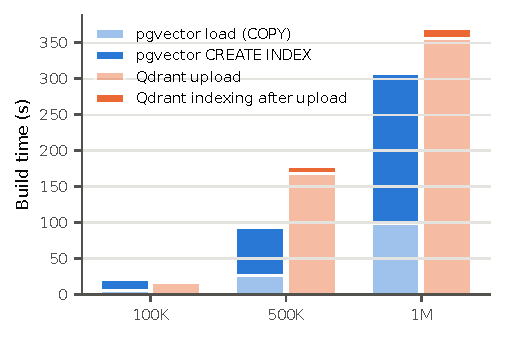
\includegraphics[width=\columnwidth]{figures/build_time.pdf}
  \caption{Build time by phase, mean of three builds on one node. Light segments: data
  ingestion (pgvector \texttt{COPY}, Qdrant upload); dark segments: index construction
  after ingestion.}
  \label{fig:build}
\end{figure}

The size of pgvector's index does not change with $M$. At 500K it is 3.81\,GiB for
$M=16$, 32 and 64. A 1024-dimensional element takes about 4\,KB, so a second element does
not fit on the same 8\,KB page. The index therefore uses one page per vector, and the
neighbor lists fit in the space that is left.

\subsection{Latency at Matched Recall}

Figure~\ref{fig:recall} shows the recall--latency curves, end to end in the top row and
engine side in the bottom row. Table~\ref{tab:matched} reads the curves at two recall
targets. At every scale and target, Qdrant's engine is 3.0--3.9$\times$ faster than
pgvector's, and its p99 latency is closer to its mean. End-to-end results depend on the
client path. With gRPC-lean, Qdrant remains 1.7--3.3$\times$ faster. With the official
gRPC client the advantage drops to 0.8--2.3$\times$, and with REST to 0.5--1.7$\times$.
At Recall@10 = 0.90, a Qdrant user on REST waits longer than a pgvector user at every
scale. Qdrant moves ahead over REST only at high recall and large scale, where pgvector's
engine time is the larger part of the total.

\begin{figure*}[t]
  \centering
  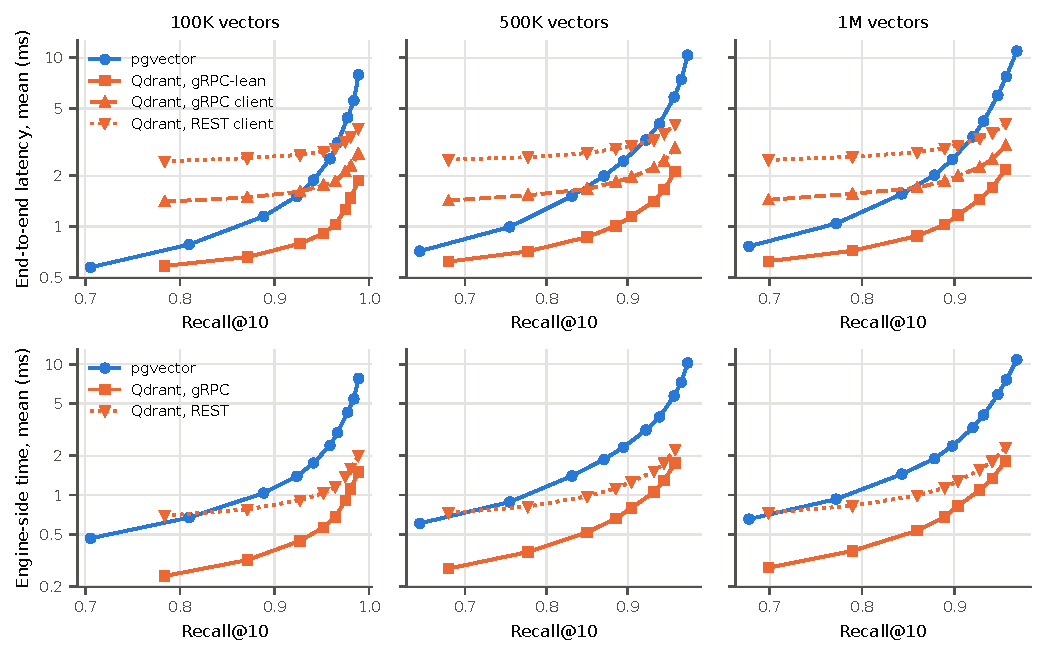
\includegraphics[width=\textwidth]{figures/recall_latency.pdf}
  \caption{Recall@10 against mean latency, end to end (top) and engine side (bottom),
  one point per $ef$ (mean of three passes over 1{,}677 queries). gRPC-lean and the
  official gRPC client share the same engine path.}
  \label{fig:recall}
\end{figure*}

\begin{table*}[t]
  \caption{Latency at matched Recall@10 (ms, log-linear interpolation between swept
  $ef$ values; three passes each, coefficient of variation of the mean at most 6\%).
  ``eng.'' is engine-side time.}
  \label{tab:matched}
  \small
  \begin{tabular}{rr|rrr|rrr|r|rr|r}
    \toprule
     & & \multicolumn{3}{c|}{pgvector} & \multicolumn{3}{c|}{Qdrant gRPC-lean} &
       gRPC client & \multicolumn{2}{c|}{REST client} & engine \\
    $N$ & Recall & mean & p99 & eng. & mean & p99 & eng. & mean & mean & eng. & speedup \\
    \midrule
    100K & 0.90 & 1.25 & 2.06 & 1.14 & 0.72 & 0.88 & 0.38 & 1.55 & 2.60 & 0.84 & 3.0$\times$ \\
    100K & 0.95 & 2.18 & 3.26 & 2.05 & 0.90 & 1.11 & 0.56 & 1.74 & 2.78 & 1.03 & 3.7$\times$ \\
    500K & 0.90 & 2.58 & 4.38 & 2.45 & 1.11 & 1.48 & 0.76 & 1.93 & 2.98 & 1.23 & 3.2$\times$ \\
    500K & 0.95 & 5.06 & 7.86 & 4.93 & 1.81 & 2.38 & 1.45 & 2.62 & 3.73 & 1.93 & 3.4$\times$ \\
    1M & 0.90 & 2.57 & 4.48 & 2.44 & 1.13 & 1.51 & 0.78 & 1.95 & 2.99 & 1.24 & 3.1$\times$ \\
    1M & 0.95 & 6.46 & 9.84 & 6.32 & 1.98 & 2.64 & 1.62 & 2.81 & 3.87 & 2.10 & 3.9$\times$ \\
    \bottomrule
  \end{tabular}
\end{table*}

Comparing the two rows of Figure~\ref{fig:recall} shows where the client cost arises.
The difference between end-to-end and engine time is about 0.1\,ms for psycopg and
0.35\,ms for gRPC-lean, and 1.1--1.2\,ms for the official gRPC client. Most of the time a
Python user of the official client waits is therefore spent in the client. REST also
adds work on the server. At the same $ef$, Qdrant's engine-side time over REST is
0.4--0.5\,ms higher than over gRPC, which we attribute to JSON parsing and
serialization.

\subsection{Concurrency}

Figure~\ref{fig:throughput} shows closed-loop throughput at matched recall, that is, at
the smallest swept $ef$ reaching Recall@10 $\geq 0.95$. Both systems scale almost
linearly until the number of clients reaches the 8 server cores. After that they level
off, with the server using 7.9 of its 8 cores. In PostgreSQL, 97--100\% of the sampled
backend states are on CPU and lock waits are at most 0.5\%, so throughput is limited by
computation and not by contention. At the plateau Qdrant serves 1.68$\times$ pgvector's
throughput at 100K (4{,}933 vs.\ 2{,}938\,qps), 1.19$\times$ at 500K (1{,}531 vs.\
1{,}288\,qps) and 1.55$\times$ at 1M (1{,}472 vs.\ 952\,qps, both at Recall@10 = 0.956).
The official gRPC client reaches the same plateau as gRPC-lean, since 28 client cores
are enough to absorb its extra cost. REST levels off 10--28\% lower because JSON
handling also uses server CPU. At 100K a query costs 1.8--2.3\,ms of server CPU over
REST and 1.2--1.7\,ms over gRPC.

\begin{figure*}[t]
  \centering
  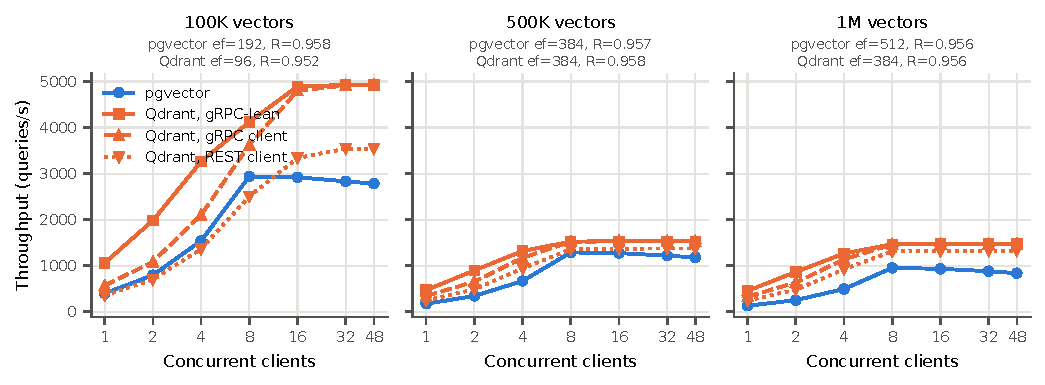
\includegraphics[width=\textwidth]{figures/throughput.pdf}
  \caption{Closed-loop throughput against concurrent client processes at matched recall,
  8 server cores. Panel subtitles give each system's $ef$ and Recall@10.}
  \label{fig:throughput}
\end{figure*}

The two systems behave differently when there are more clients than cores. pgvector
runs one backend process per connection, so 48 clients mean 48 runnable processes on
8 cores. Its throughput drops 5--12\% below the peak, the CPU time per query rises (from
8.3 to 9.5\,ms at 1M), and p99 latency grows to 2.3--3.7$\times$ the mean (130\,ms at
1M). Qdrant queues requests for a fixed pool of search threads. Its throughput stays at
the plateau and its p99 stays within 1.06--1.38$\times$ of the mean (35\,ms at 1M). With
a single client, Qdrant keeps 1.5--2.3 cores busy because it searches its four segments
in parallel. This lowers single-query latency, but it does not raise throughput once all
cores are busy.

Engine-side times cannot be compared directly between the systems under load. Qdrant's
request time includes the wait for a free search thread, while a PostgreSQL backend
waits in the operating system's run queue before its statement starts, which the
statement time does not include. For this reason we compare engine-side times only at
$C=1$ and use end-to-end latency under load.
\todo{Hardware counters per client path.}

\subsection{HNSW Parameters}

Table~\ref{tab:hnsw} repeats the 500K comparison with eight construction settings. In
all of them Qdrant's engine is 3.4--4.5$\times$ faster at Recall@10 = 0.95, and its
throughput plateau at matched recall is 1.2--2.1$\times$ higher. The gap is therefore not
specific to $M=16$, $ef_{construction}=64$. Denser graphs let both systems reach higher
recall. For pgvector they also increase build time roughly in line with the extra work,
and \texttt{CREATE INDEX} grows from 75\,s to 554\,s across the grid. Qdrant's total build
time stays between 135 and 166\,s, because indexing overlaps with the upload and the
upload takes longer.

\begin{table}[h]
  \caption{HNSW construction parameters at 500K. Engine time (ms) at Recall@10 = 0.95;
  peak throughput (qps) at the matched-recall $ef$; pgvector index-build and Qdrant total
  build time (s).}
  \label{tab:hnsw}
  \small
  \begin{tabular}{rr|rrr|rrr}
    \toprule
     & & \multicolumn{3}{c|}{pgvector} & \multicolumn{3}{c}{Qdrant} \\
    $M$ & $ef_c$ & index s & eng. & qps & build s & eng. & qps \\
    \midrule
    16 & 64 & 75 & 4.81 & 1021 & 143 & 1.40 & 1241 \\
    16 & 128 & 135 & 3.28 & 1735 & 165 & 0.89 & 2840 \\
    16 & 256 & 209 & 2.46 & 2682 & 135 & 0.69 & 3976 \\
    32 & 64 & 136 & 5.03 & 1157 & 152 & 1.36 & 2017 \\
    32 & 128 & 188 & 3.51 & 1932 & 148 & 0.88 & 2520 \\
    32 & 256 & 282 & 2.93 & 1806 & 146 & 0.84 & 3422 \\
    64 & 128 & 352 & 4.25 & 1126 & 166 & 0.95 & 2411 \\
    64 & 256 & 554 & 3.55 & 1829 & 143 & 0.90 & 3028 \\
    \bottomrule
  \end{tabular}
\end{table}

Because the matched-recall $ef$ is the smallest swept value reaching 0.95, the two
systems' throughput is measured at slightly different recall (pgvector 0.955--0.972,
Qdrant 0.950--0.967). pgvector's engine time does not decrease steadily with graph
density. The $(32,64)$ graph is slower than $(16,64)$, and $(64,128)$ is slower than
$(32,128)$, which may reflect variation in graph quality from one build to the next.
\todo{Repeat builds to quantify graph-quality variance.}

\subsection{Dimensionality}
\label{sec:dims}

Figure~\ref{fig:dims} varies the dimension from 128 to 1024 at 100K vectors. Qdrant is run
twice at each dimension, once with the default optimizer settings and once with the
indexing threshold lowered to 1\,KB so that every segment gets an HNSW graph. When every
segment is indexed, Qdrant's engine time grows smoothly with $d$, from 0.21 to 0.44\,ms at
$ef=64$, and pgvector's grows from 0.77 to 1.05\,ms. At Recall@10 = 0.90 Qdrant's engine
is 2.9--5.3$\times$ faster across dimensions, and the gap is largest at $d=128$. With the
default settings, Qdrant leaves 1.7--5.8\% of the vectors unindexed at five of the eight
dimensions. This happens whenever the last segment ends up smaller than the 20\,MB
threshold, and those vectors are then scanned exhaustively. At these dimensions the
engine time rises by up to 1.9$\times$ and recall also rises, because part of each answer
comes from an exact scan. The resulting saw-tooth curve is the ``384-dimension anomaly''
we saw in our first measurements. It comes from the optimizer state, and SIMD alignment
does not explain it.

\begin{figure*}[t]
  \centering
  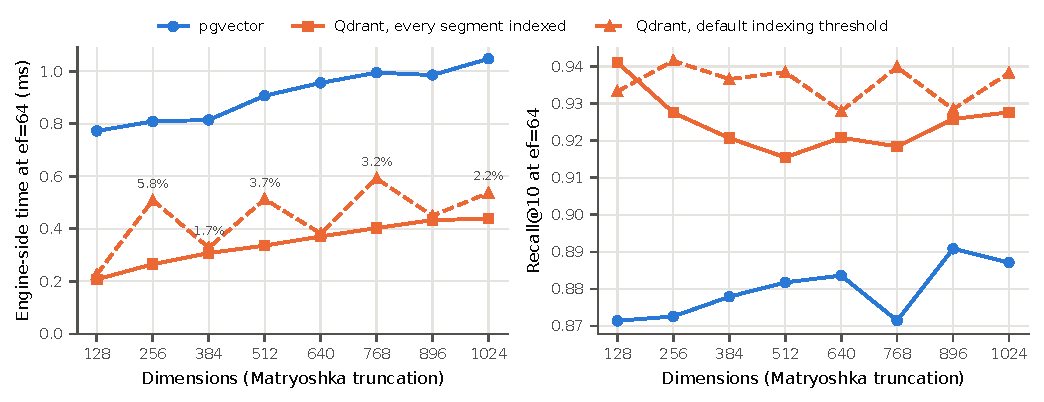
\includegraphics[width=\textwidth]{figures/dimensionality.pdf}
  \caption{Engine-side time (left) and Recall@10 (right) at $ef=64$ against dimension,
  100K vectors. Labels give the share of vectors Qdrant left unindexed with its default
  indexing threshold.}
  \label{fig:dims}
\end{figure*}

\subsection{Memory Pressure}
\label{sec:memory}

\textbf{Buffer pool.} Table~\ref{tab:sb} shows pgvector at 1M vectors with four sizes of
shared buffers. Nothing in these runs is read from disk. The machine has far more memory
than the data, and a page that is not in shared buffers is copied from the operating
system's page cache. Even so, the buffer pool size changes the results considerably.
With 32\,GB the whole index is in shared buffers, every block access is a hit, and the
sampled backends spend all their time on CPU. With the default 128\,MB, 82\% of the
block accesses miss and are read from the page cache, the engine time at $ef=64$ rises
from 1.41 to 3.82\,ms (2.7$\times$), and throughput at $C=8$ falls from 4{,}954 to
1{,}648\,qps (3.0$\times$). At $ef=512$, which reaches Recall@10 = 0.956, the effect is
the same: 7.52 against 20.50\,ms and 978 against 307\,qps.

Each read from the page cache costs about 3\,$\mu$s per 8\,KiB block in every
configuration, and the read time that PostgreSQL records accounts for 86--108\% of the
extra engine time. The copies are also CPU work, which is why throughput falls along
with latency. The server CPU time per query at $C=8$ grows from 1.52\,ms with 32\,GB to
4.68\,ms with 128\,MB. With 32 clients, backends also wait on the buffer mapping lock
(\texttt{LWLock:BufferMapping}, 41\% of samples with 128\,MB), and p99 latency at
$ef=64$ grows from 15.7 to 65.9\,ms. A 4\,GB buffer pool, about half the index, recovers
part of the loss: 77\% of the accesses hit and the engine time is 2.33\,ms.

This confirms, with direct measurement, the buffer-pool explanation that we could only
suggest in our first measurements. It also means that the size of the gap between the
two systems depends on how PostgreSQL is configured. Our main results use 32\,GB of
shared buffers. With PostgreSQL's default, pgvector's engine time would be about
2.7$\times$ longer, and Qdrant's engine advantage at matched recall correspondingly
larger.

\begin{table}[h]
  \caption{pgvector at 1M vectors with different \texttt{shared\_buffers}, no memory limit
  (whole index in the OS page cache). Hit ratio and blocks read per query at $ef=64$;
  engine time (ms) and throughput at $C=8$ (qps) at $ef=64$ (Recall@10 = 0.84) and
  $ef=512$ (0.956).}
  \label{tab:sb}
  \small
  \begin{tabular}{r|rr|rr|rr}
    \toprule
     & & & \multicolumn{2}{c|}{$ef=64$} & \multicolumn{2}{c}{$ef=512$} \\
    shared buffers & hit & reads & eng. & qps & eng. & qps \\
    \midrule
    32\,GB & 1.00 & 0 & 1.41 & 4954 & 7.52 & 978 \\
    4\,GB & 0.77 & 273 & 2.33 & 2456 & 12.99 & 506 \\
    1\,GB & 0.34 & 758 & 3.73 & 1771 & 20.06 & 329 \\
    128\,MB & 0.18 & 939 & 3.82 & 1648 & 20.50 & 307 \\
    \bottomrule
  \end{tabular}
\end{table}

\textbf{Memory limits.} Table~\ref{tab:caps} shows both systems after their files are
evicted from the page cache and the server is restarted under a memory limit. The data
on disk differs in size. pgvector's index takes 7.61\,GiB, while Qdrant's whole storage,
vectors and graph together, takes 3.94\,GiB. A 1024-dimensional vector fills about half
of an 8\,KiB page, and pgvector stores one graph element per page
(Section~\ref{sec:build}), so it reads and caches about twice as many bytes for the same
vectors.

The first pass after a cold start is slow for both systems because each query waits for
random reads from the spinning disk. pgvector needs 1.7--1.9\,s per query at $ef=64$,
reading about 750 blocks per query, and Qdrant needs 1.0--1.2\,s. After this pass the
300 measured queries have touched only part of the data, and that part fits in the
larger limits. With 8\,GB or more, both systems are back to their in-memory latency by
the first concurrency window. With 4\,GB, Qdrant is also back to 0.86\,ms, but pgvector
is still reading from disk at 327\,ms per query with one client, and reaches in-memory
throughput only during the 32-client window. With 2\,GB, neither system stops reading
from disk. pgvector serves 3\,qps with 32 clients and Qdrant 20\,qps, with mean latencies
of 9.7 and 1.6\,s. Part of pgvector's disadvantage at this limit is that its 1\,GB of
shared buffers counts against the same limit, which leaves less memory for the page
cache.

Without a limit, Qdrant's memory-mapped files were also not in the page cache after the
build, so its first pass was as slow as under the limits. pgvector's files were still
cached from the build. This is why the two ``none'' rows differ.

\begin{table}[h]
  \caption{Cold start under cgroup memory limits, 1M vectors, $ef=64$, first 300 queries.
  ``First pass'': mean latency of the first measured pass after a restart with an
  evicted cache (ms). $C=1$: mean latency in the first concurrency window (ms). $C=32$:
  throughput in the last window (qps). pgvector uses 1\,GB of shared buffers; Qdrant
  memory-maps vectors and graph.}
  \label{tab:caps}
  \small
  \begin{tabular}{r|rrr|rrr}
    \toprule
     & \multicolumn{3}{c|}{pgvector} & \multicolumn{3}{c}{Qdrant} \\
    limit & first pass & $C=1$ & $C=32$ & first pass & $C=1$ & $C=32$ \\
    \midrule
    none & 3.91 & 3.63 & 5552 & 1042 & 0.85 & 5867 \\
    16\,GB & 1725 & 3.62 & 5087 & 1040 & 0.86 & 5868 \\
    8\,GB & 1698 & 3.63 & 5592 & 1042 & 0.86 & 5862 \\
    4\,GB & 1698 & 327 & 5000 & 1039 & 0.86 & 5866 \\
    2\,GB & 1865 & 1436 & 3 & 1209 & 866 & 20 \\
    \bottomrule
  \end{tabular}
\end{table}

%% =============================================================
\section{Discussion}
%% =============================================================

When the working set fits in memory, Qdrant's engine answers queries 3--4$\times$ faster
than pgvector's at equal recall, from 100K to 1M vectors and for every HNSW configuration
and dimension we tested. It also uses less CPU per query at saturation. For an
application, however, the client matters about as much as the engine. Through Qdrant's
official REST client, pgvector was the faster system at Recall@10 = 0.90 at every scale we
measured. A team choosing between the two should therefore consider which client and
protocol it will use, and not only which engine is faster.

Under load, both systems are limited by CPU and not by locking. They differ in how they
handle overload. Qdrant's fixed thread pool keeps latency predictable when there are more
clients than cores. pgvector's process-per-connection model loses some throughput and
develops a long latency tail in that situation, so a deployment would benefit from a
connection pooler sized to the number of cores. With its build parallelism configured,
pgvector built its index faster than Qdrant at 500K and 1M on the same node, which
reverses the large build-time advantage for Qdrant that our first measurements showed.
Build times also varied considerably between nodes, so single build measurements on a
shared cluster should be treated with care.

Memory configuration matters as much as the choice of system. With PostgreSQL's
default buffer pool, pgvector reads most index pages from the operating system's page
cache, and this alone made it 2.7$\times$ slower in our runs, with no disk access at all.
Anyone deploying pgvector, or benchmarking it, should size \texttt{shared\_buffers} to
hold the HNSW index. When the index does not fit in memory at all, pgvector is at a
disadvantage at 1024 dimensions, because its page layout roughly doubles the size of the
data it has to read and cache. On our spinning disks a cold query took one to two
seconds in both systems, so neither is usable out of core on such hardware. Qdrant
recovered with a smaller memory limit and stayed faster under the tightest one.

On methodology, the confounders in Table~\ref{tab:confounders} reversed all three main
results of our first measurements. The planner fallback is worth noting separately,
because pgvector can stop using the HNSW index for TOASTed vectors without any warning.
The query still returns correct results, only much more slowly. Benchmarks, and also
applications in production, should check the query plan rather than assume the index is
used.

\subsection{Threats to Validity}

\textbf{Single node, single client language.} Both systems run on a single node and are
queried from Python. Clients written in compiled languages would reduce the client's
share of latency further, and gRPC-lean gives an approximate lower bound for it.

\textbf{Shared infrastructure.} Each node runs only our job, but the parallel file
system and the interconnect are shared with other users. Database files are kept on
node-local disk, and every result records the node's load and any other jobs on it.
Query measurements run from memory and are not affected by the disk, but build times
are, so all build times we report come from a single node.

\textbf{Configuration.} We tune PostgreSQL's memory settings for an in-memory working
set and leave Qdrant at its defaults, apart from $ef_{construction}$. Experiments E2 and
E4 vary the parameters most likely to change the conclusions. E4 shows that with
PostgreSQL's default \texttt{shared\_buffers}, pgvector would compare considerably worse
than in our main results.

\textbf{Memory-limit runs.} The memory-limit runs use a spinning disk, one pass over 300
queries and a single repetition, and they measure a warm-up path from a cold cache
rather than a steady state. The results show how each system starts from a cold cache
and which limits its working set fits in. They do not show performance on SSDs, where
a random read takes a small fraction of the 4.8\,ms we measured. pgvector's shared buffers count against its
memory limit, while Qdrant has no equivalent fixed allocation.

\textbf{Single embedding model and corpus.} All experiments use Cohere v3 embeddings of
MS MARCO. Matryoshka truncation is only an approximation of models that natively produce
lower-dimensional embeddings.

\textbf{Engine-side timing.} The two systems measure engine time at different points
(statement execution in PostgreSQL, request handling in Qdrant), so we use it to break
down latency only at $C=1$.

%% =============================================================
\section{Conclusion}
%% =============================================================

We compared pgvector and Qdrant, two systems built on the same HNSW index, under
conditions designed to remove the usual sources of bias: dedicated nodes, real queries,
comparison at matched recall, separate engine and client times, and builds measured to
completion. With the data in memory, Qdrant's engine is 3--4$\times$ faster at equal
recall across scales, HNSW settings and dimensions, and it keeps tail latency under
control when overloaded. The advantage an application actually sees, however, depends on
the client path. Through the official REST client it disappears at moderate recall.
pgvector builds its index faster than Qdrant at 500K and 1M once build parallelism is
set, and its performance depends strongly on the buffer pool. With the default setting it is
2.7$\times$ slower even when nothing is read from disk. Under memory limits, pgvector's
one-page-per-vector layout doubles the data it has to read, and Qdrant tolerates tighter
limits.

Several of these results reverse what a simpler benchmark of the same two systems
showed, and some of the reasons are easy to miss: an indexing threshold that leaves
data unindexed while the collection reports ready, a planner cost model that abandons
the index without a warning, and client libraries that cost more time than the search
itself. We hope the list of confounders and the open harness make future comparisons of
vector stores easier to trust. Natural next steps are filtered (hybrid) search,
workloads that mix reads and writes, SSD-backed out-of-core runs, and clients in compiled
languages.

\begin{acks}
The numerical calculations reported in this paper were fully performed at TÜBİTAK
ULAKBİM, High Performance and Grid Computing Center (TRUBA resources).
\todo{Check the exact acknowledgement text required by TRUBA.}
\end{acks}

\begin{thebibliography}{00}

\bibitem{malkov2018}
Y.~A. Malkov and D.~A. Yashunin, ``Efficient and robust approximate nearest
neighbor search using hierarchical navigable small world graphs,''
\textit{IEEE Transactions on Pattern Analysis and Machine Intelligence},
vol.~42, no.~4, pp.~824--836, 2020.

\bibitem{zhang2024}
Y.~Zhang, S.~Liu, and J.~Wang, ``Are there fundamental limitations in supporting
vector data management in relational databases? A case study of PostgreSQL,'' in
\textit{Proc.\ 40th IEEE International Conference on Data Engineering (ICDE)}, 2024.
\todo{verify author list}

\bibitem{pan2024survey}
J.~J. Pan, J.~Wang, and G.~Li, ``Survey of vector database management systems,''
\textit{The VLDB Journal}, vol.~33, pp.~1591--1615, 2024. \todo{verify pages}

\bibitem{aumuller2020}
M.~Aumüller, E.~Bernhardsson, and A.~Faithfull, ``ANN-Benchmarks: A benchmarking tool
for approximate nearest neighbor algorithms,'' \textit{Information Systems}, vol.~87,
101374, 2020.

\bibitem{pgvector}
pgvector, ``Open-source vector similarity search for PostgreSQL,'' version 0.8.6.
\url{https://github.com/pgvector/pgvector}

\bibitem{qdrant}
Qdrant, ``Qdrant documentation,'' version 1.19. \url{https://qdrant.tech/documentation/}

\bibitem{postgres_docs}
PostgreSQL Global Development Group, ``PostgreSQL 17 Documentation.''
\url{https://www.postgresql.org/docs/17/}

\bibitem{cohere2024}
Cohere, ``Introducing Embed v3,'' Cohere Blog, 2023.
\url{https://cohere.com/blog/introducing-embed-v3}

\bibitem{msmarco}
P.~Bajaj et al., ``MS MARCO: A human generated machine reading comprehension
dataset,'' arXiv:1611.09268, 2016.

\end{thebibliography}

\end{document}
